\chapter{Semaine 2 : Conception de l'Interface d'Accueil}
\thispagestyle{fancy}

La deuxième semaine du stage a été consacrée au développement de l'interface d'accueil de la plateforme e-learning. Cette étape était cruciale pour établir l'identité visuelle du projet et créer une première impression positive auprès des utilisateurs.

\section{Conception de la Page d'Accueil}

La page d'accueil a été conçue pour présenter clairement la valeur ajoutée de la plateforme et inciter les utilisateurs à s'inscrire. Plusieurs sections ont été développées pour structurer l'information de manière efficace.

\subsection{Hero Section}
La section principale (Hero Section) a été conçue pour capturer immédiatement l'attention des visiteurs avec un message clair et une incitation à l'action.

\begin{figure}[h!]
  \centering
  
\includegraphics[width=0.9\textwidth,keepaspectratio]{week_2_img/last_and_improved_hero_section_withe_3d_effects_etc.png}
  \caption{\textbf{Hero Section améliorée} de la page d'accueil avec effets 3D et animations interactives.}
  \label{fig:hero_section_improved}
\end{figure}

Les éléments clés de cette section comprennent :
\begin{itemize}
  \item Un titre accrocheur qui met en avant la proposition de valeur principale
  \item Un sous-titre explicatif sur les avantages de la plateforme
  \item Un bouton d'appel à l'action bien visible pour l'inscription
  \item Une illustration moderne avec des effets 3D représentant le concept d'apprentissage en ligne
  \item Un design responsive qui s'adapte à tous les types d'écrans
  \item Des animations interactives qui s'activent au survol ou au défilement
\end{itemize}

\subsection{Section "Where We Are"}
Une section spécifique a été développée pour illustrer la portée géographique et l'influence de la plateforme, renforçant ainsi sa crédibilité auprès des utilisateurs potentiels.

\begin{figure}[h!]
  \centering
  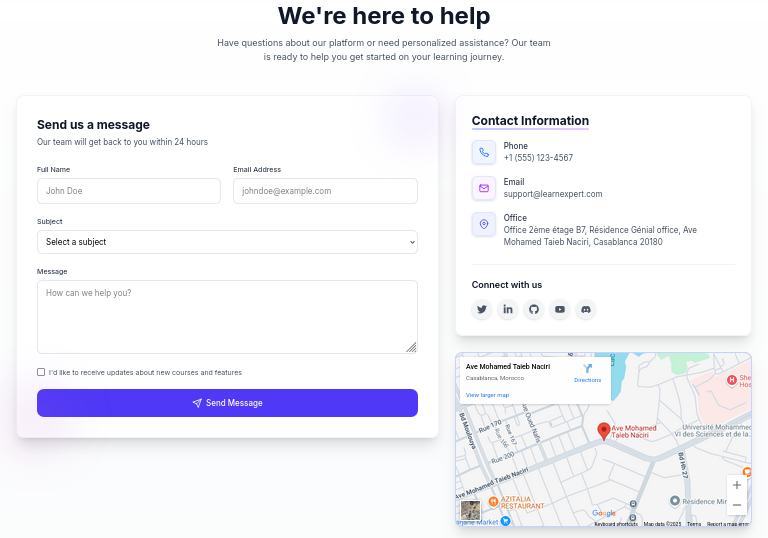
\includegraphics[width=0.9\textwidth,keepaspectratio]{week_2_img/where_we_are_section.png}
  \caption{\textbf{Section "Where We Are"} présentant la présence globale de la plateforme.}
  \label{fig:where_we_are}
\end{figure}

Cette section met en évidence :
\begin{itemize}
  \item Une carte interactive montrant la présence internationale
  \item Des statistiques sur le nombre d'utilisateurs par région
  \item Des témoignages d'utilisateurs de différentes zones géographiques
  \item Une visualisation de la croissance de la communauté mondiale
\end{itemize}

\subsection{Sections de Fonctionnalités}
Pour mettre en évidence les principales fonctionnalités de la plateforme, trois sections distinctes ont été développées, chacune mettant en avant un aspect spécifique de l'offre.

\begin{figure}[h!]
  \centering
  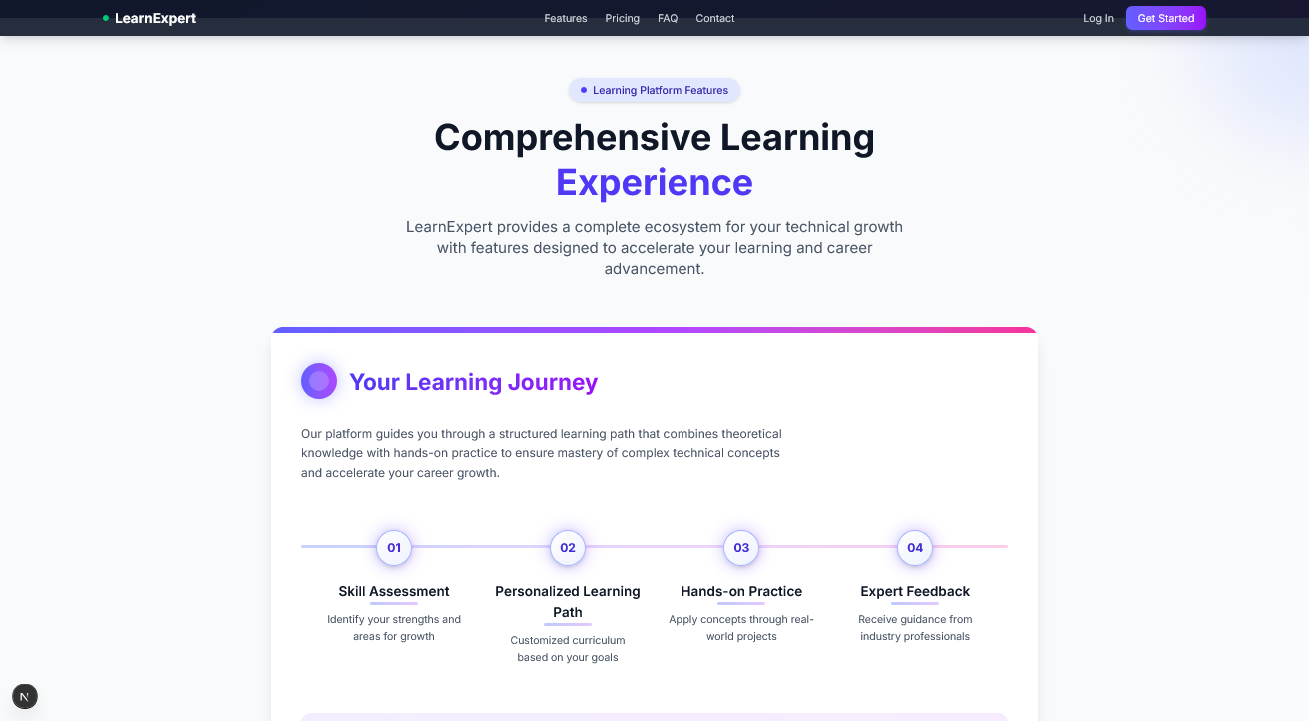
\includegraphics[width=0.9\textwidth,keepaspectratio]{week_2_img/featchersection_1.png}
  \caption{\textbf{Première section de fonctionnalités} présentant les cours en ligne.}
  \label{fig:features_section_1}
\end{figure}

\begin{figure}[h!]
  \centering
  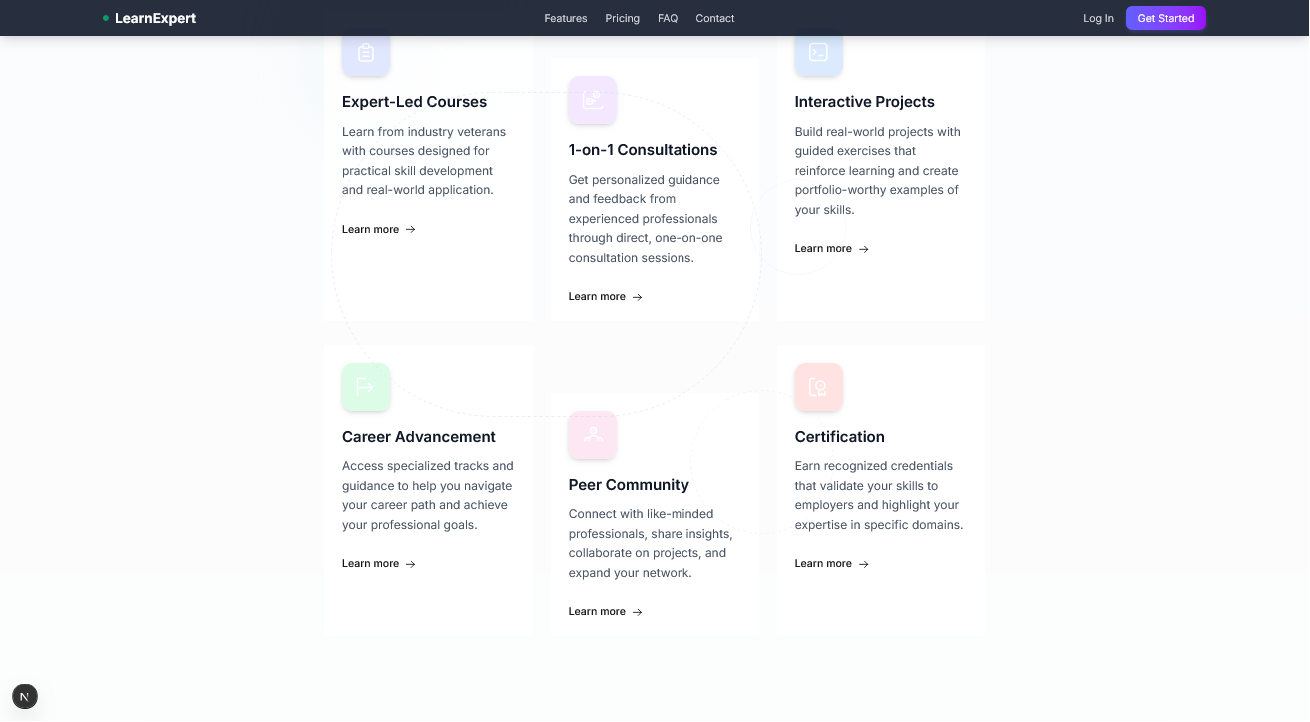
\includegraphics[width=0.9\textwidth,keepaspectratio]{week_2_img/fetchersection_2.png}
  \caption{\textbf{Deuxième section de fonctionnalités} mettant en avant les services de consultation.}
  \label{fig:features_section_2}
\end{figure}

\begin{figure}[h!]
  \centering
  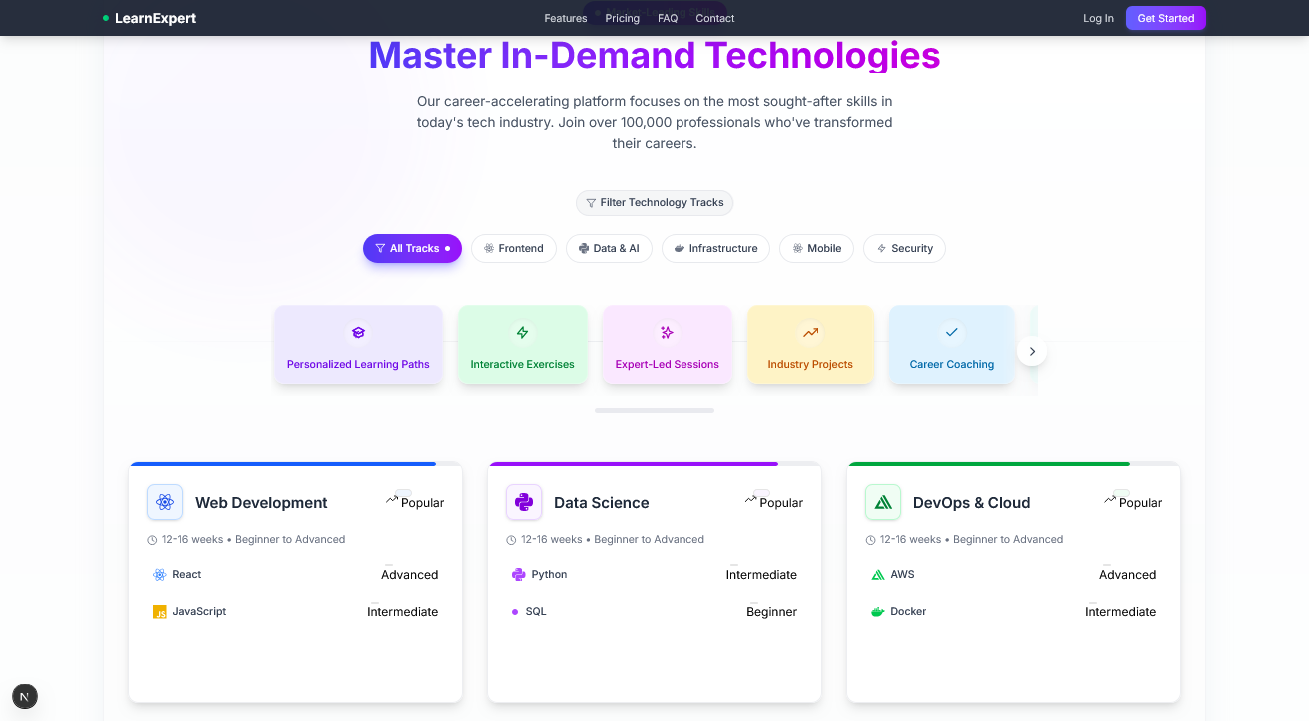
\includegraphics[width=0.9\textwidth,keepaspectratio]{week_2_img/fetchersection_3.png}
  \caption{\textbf{Troisième section de fonctionnalités} présentant les outils d'analyse et de suivi.}
  \label{fig:features_section_3}
\end{figure}

Chaque section de fonctionnalités comprend :
\begin{itemize}
  \item Une illustration ou icône représentative
  \item Un titre explicite de la fonctionnalité
  \item Une description détaillée des avantages
  \item Une mise en page alternée (image à gauche, texte à droite et inversement) pour créer un rythme visuel
\end{itemize}

\subsection{Section FAQ}
Pour répondre aux questions fréquentes des utilisateurs potentiels, une section FAQ interactive a été développée avec un système d'accordéon permettant de masquer/afficher les réponses.

\begin{figure}[h!]
  \centering
  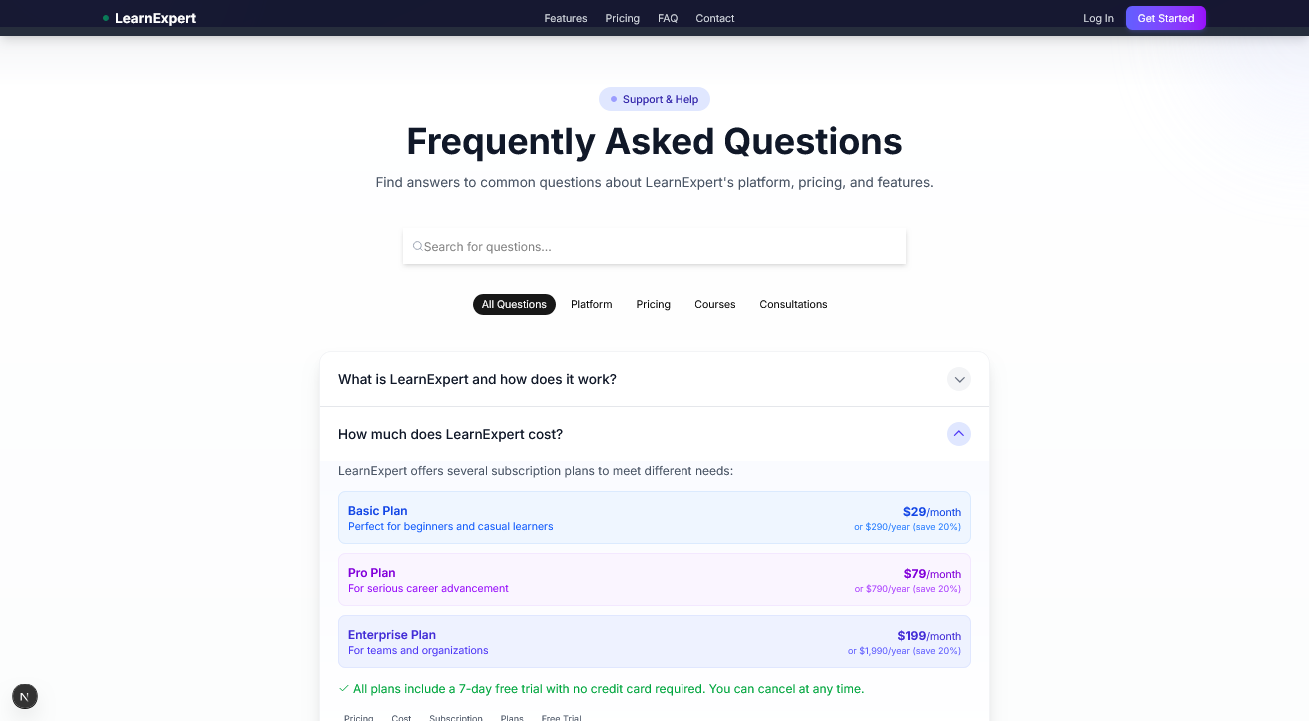
\includegraphics[width=0.9\textwidth,keepaspectratio]{week_2_img/faqsection.png}
  \caption{\textbf{Section FAQ} avec questions-réponses interactives.}
  \label{fig:faq_section}
\end{figure}

\subsection{Appel à l'Action Final}
Une seconde section d'appel à l'action a été ajoutée en bas de page pour inciter les utilisateurs ayant parcouru l'ensemble du contenu à s'inscrire.

\begin{figure}[h!]
  \centering
  
\includegraphics[width=0.9\textwidth,keepaspectratio]{week_2_img/second_call_of_action.png}
  \caption{\textbf{Section d'appel à l'action finale} incitant à l'inscription.}
  \label{fig:final_cta}
\end{figure}

\subsection{Barre de Navigation et Pied de Page}
La barre de navigation et le pied de page ont été conçus pour offrir un accès facile aux différentes sections du site et renforcer la crédibilité de la plateforme.

\begin{figure}[h!]
  \centering
  
\includegraphics[width=0.9\textwidth,keepaspectratio]{week_2_img/navbar.png}
  \caption{\textbf{Barre de navigation} avec les liens vers les principales sections.}
  \label{fig:navbar}
\end{figure}

\begin{figure}[h!]
  \centering
  
\includegraphics[width=0.9\textwidth,keepaspectratio]{week_2_img/foter.png}
  \caption{\textbf{Pied de page} avec informations légales et liens supplémentaires.}
  \label{fig:footer}
\end{figure}

\section{Mise en Place du Système de Paiement}

Un système de paiement sécurisé a également été intégré à la plateforme pour permettre l'achat d'abonnements et de services.

\begin{figure}[h!]
  \centering
  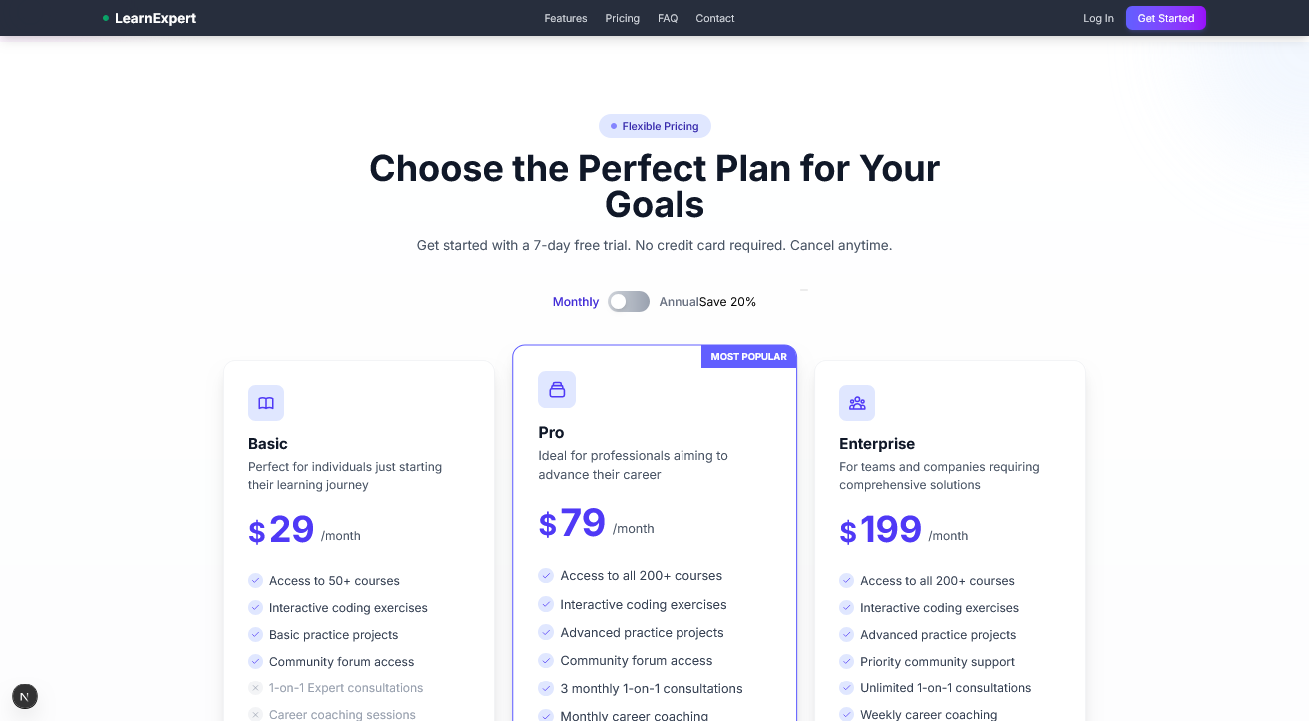
\includegraphics[width=0.9\textwidth,keepaspectratio]{week_2_img/payment_1.png}
  \caption{\textbf{Interface de paiement} pour les abonnements et services.}
  \label{fig:payment}
\end{figure}

Les fonctionnalités clés du système de paiement incluent :
\begin{itemize}
  \item Sélection de différentes formules d'abonnement
  \item Interface de saisie des informations de carte bancaire sécurisée
  \item Intégration avec un service de paiement externe (Stripe)
  \item Confirmation de paiement et génération de facture automatique
  \item Gestion des abonnements récurrents et des annulations
\end{itemize}

\section{Technologies Utilisées}

Pour le développement front-end de cette page d'accueil, les technologies suivantes ont été utilisées :
\begin{itemize}
  \item \textbf{Next.js :} Framework React pour le rendu côté serveur et la génération de sites statiques
  \item \textbf{Tailwind CSS :} Framework CSS utilitaire pour un design responsive et personnalisable
  \item \textbf{Framer Motion :} Bibliothèque d'animations pour ajouter des transitions et effets visuels
  \item \textbf{React Hook Form :} Gestion des formulaires avec validation
  \item \textbf{TypeScript :} Pour un code plus robuste avec typage statique
\end{itemize}

\section{Optimisations et Performances}

Une attention particulière a été portée à l'optimisation des performances :
\begin{itemize}
  \item Utilisation de l'optimisation d'images intégrée à Next.js
  \item Lazy loading des images et composants non critiques
  \item Minification du code CSS et JavaScript
  \item Mise en cache efficace pour réduire les temps de chargement
  \item Design responsive optimisé pour tous les appareils
\end{itemize}

\section{Méthodologie de Conception}

Le processus de conception de l'interface a suivi une approche méthodique :

\subsection{Analyse des Besoins et Recherche}
\begin{itemize}
  \item Étude des plateformes concurrentes pour identifier les meilleures pratiques
  \item Analyse des besoins des utilisateurs cibles
  \item Définition des objectifs principaux de la page d'accueil
\end{itemize}

\subsection{Wireframing et Prototypage}
\begin{itemize}
  \item Création de wireframes simples pour définir la structure de la page
  \item Développement de prototypes interactifs avec Figma
  \item Tests utilisateurs préliminaires pour valider les concepts
\end{itemize}

\subsection{Développement Itératif}
\begin{itemize}
  \item Implémentation progressive des différentes sections
  \item Sessions quotidiennes de feedback avec l'équipe
  \item Améliorations continues basées sur les retours
\end{itemize}

\section{Résultats et Impacts}

La conception de cette interface d'accueil a établi une base solide pour le développement des autres composants de la plateforme e-learning, en définissant une identité visuelle cohérente et en présentant clairement la proposition de valeur aux utilisateurs potentiels. 

\section{Conclusion}

Cette deuxième semaine de stage a été très productive, avec des avancées significatives dans le développement frontend de la plateforme. La création d'une page d'accueil attrayante et fonctionnelle constitue une étape importante du projet. Les différentes sections développées (Hero Section améliorée, Where We Are, fonctionnalités, FAQ, etc.) permettent de présenter efficacement la valeur ajoutée de la plateforme et d'inciter les utilisateurs à s'inscrire. Les prochaines étapes se concentreront sur le développement des interfaces internes pour les utilisateurs connectés et l'intégration des fonctionnalités backend. 